\documentclass{article}

\usepackage{fancyhdr}
\usepackage{extramarks}
\usepackage{amsmath}
\usepackage{amsthm}
\usepackage{amsfonts}
\usepackage{tikz}
\usepackage[plain]{algorithm}
\usepackage{algpseudocode}
\usepackage{enumerate}
\usepackage{amssymb}
\usepackage[margin=1in]{geometry}

\newcommand{\st}{~\mid~}
\newcommand{\ind}{$~~~$}
\usepackage{xcolor}

\graphicspath{ {./../images} }

\usetikzlibrary{automata,positioning}

%
% Basic Document Settings
%

\topmargin=-0.45in
\evensidemargin=0in
\oddsidemargin=0in
\textwidth=6.5in
\textheight=9.0in
\headsep=0.25in

\linespread{1.1}

\pagestyle{fancy}
\lhead{\hmwkAuthorName}
\chead{\hmwkClass:\ \hmwkTitle}
\rhead{\firstxmark}
\lfoot{\lastxmark}
\cfoot{\thepage}

\renewcommand\headrulewidth{0.4pt}
\renewcommand\footrulewidth{0.4pt}

\setlength\parindent{0pt}
\setlength{\parskip}{5pt}

%
% Create Problem Sections
%

\newcommand{\enterProblemHeader}[1]{
    \nobreak\extramarks{}{Problem \arabic{#1} continued on next page\ldots}\nobreak{}
    \nobreak\extramarks{Problem \arabic{#1} (continued)}{Problem \arabic{#1} continued on next page\ldots}\nobreak{}
}

\newcommand{\exitProblemHeader}[1]{
    \nobreak\extramarks{Problem \arabic{#1} (continued)}{Problem \arabic{#1} continued on next page\ldots}\nobreak{}
    \stepcounter{#1}
    \nobreak\extramarks{Problem \arabic{#1}}{}\nobreak{}
}

\setcounter{secnumdepth}{0}
\newcounter{partCounter}
\newcounter{homeworkProblemCounter}
\setcounter{homeworkProblemCounter}{1}
\nobreak\extramarks{Problem \arabic{homeworkProblemCounter}}{}\nobreak{}

%
% Homework Problem Environment
%
% This environment takes an optional argument. When given, it will adjust the
% problem counter. This is useful for when the problems given for your
% assignment aren't sequential. See the last 3 problems of this template for an
% example.
%
\newenvironment{homeworkProblem}[1][-1]{
    \ifnum#1>0
        \setcounter{homeworkProblemCounter}{#1}
    \fi
    \section{Problem \arabic{homeworkProblemCounter}}
    \setcounter{partCounter}{1}
    \enterProblemHeader{homeworkProblemCounter}
}{
    \exitProblemHeader{homeworkProblemCounter}
}

%
% Homework Details
%   - Title
%   - Due date
%   - Class
%   - Section/Time
%   - Instructor
%   - Author
%

\newcommand{\hmwkTitle}{Homework\ \#3}
\newcommand{\hmwkDueDate}{Apr 24, 2024}
\newcommand{\hmwkClass}{CSE 101}
\newcommand{\hmwkClassInstructor}{Professor Jones}
\newcommand{\hmwkAuthorName}{\textbf{Ray Tsai}}
\newcommand{\hmwkPID}{A16848188}

%
% Title Page
%

\title{
    \vspace{2in}
    \textmd{\textbf{\hmwkClass:\ \hmwkTitle}}\\
    \normalsize\vspace{0.1in}\small{Due\ on\ \hmwkDueDate\ at 23:59pm}\\
    \vspace{0.1in}\large{\textit{\hmwkClassInstructor}} \\
    \vspace{3in}
}

\author{
  \hmwkAuthorName \\
  \vspace{0.1in}\small\hmwkPID
}
\date{}

\renewcommand{\part}[1]{\textbf{\large Part \Alph{partCounter}}\stepcounter{partCounter}\\}

%
% Various Helper Commands
%

% Useful for algorithms
\newcommand{\alg}[1]{\textsc{\bfseries \footnotesize #1}}

% For derivatives
\newcommand{\deriv}[1]{\frac{\mathrm{d}}{\mathrm{d}x} (#1)}

% For partial derivatives
\newcommand{\pderiv}[2]{\frac{\partial}{\partial #1} (#2)}

% Integral dx
\newcommand{\dx}{\mathrm{d}x}

% Probability commands: Expectation, Variance, Covariance, Bias
\newcommand{\Var}{\mathrm{Var}}
\newcommand{\Cov}{\mathrm{Cov}}
\newcommand{\Bias}{\mathrm{Bias}}
\newcommand*{\Z}{\mathbb{Z}}
\newcommand*{\Q}{\mathbb{Q}}
\newcommand*{\R}{\mathbb{R}}
\newcommand*{\C}{\mathbb{C}}
\newcommand*{\N}{\mathbb{N}}
\newcommand*{\prob}{\mathds{P}}
\newcommand*{\E}{\mathds{E}}

\begin{document}

\maketitle

\pagebreak

\begin{homeworkProblem}
  You are given a schedule for $n$ buses in the city. The schedule is given to you as a
  2-dimensional array $B$ of dimensions $n\times k$. Each bus has $k$ stops and each entry of the
  array is an ordered pair $B[i,j] = (S_{i,j},t_{i,j})$  which means that the $j^{th}$ stop that bus
  $i$ makes is at station $S_{i,j}$ at time $t_{i,j}$ (measured in minutes counted from the
  beginning of the day.) Each row is ordered by times (i.e., $t_{i,1}<t_{i,2}<\dots <t_{i,k}$). 

  You can transfer from bus $a$ to bus $b$ at stop $X$ if there exists entries $B[a,j] =
  (X,t_{a,j})$ and $B[b,j'] = (X,t_{b,j'})$ and $t_{a,j} < t_{b,j'}$.

  \begin{enumerate}[(a)]
  \item
  Given bus stations $X$ and $Y$ and a starting time $T$, design an algorithm that returns the
  earliest time you can reach station $Y$ from station $X$ starting any time after time $T$ using a
  sequence of transfers.

  \begin{proof}
    Let $V$ be the set of stations. Consider the following algorithm:
    \begin{quote}
      \begin{enumerate}[1.]
      \item
      {\bf for all} $v \in V$:
      \item
      \ind $time(v) = \infty$
      \item
      \ind Initialize array $schedule(v)$
      \item
      $time(X) = T$
      \item
      {\bf for each} entry in $B$:
      \item
      \ind $append(schedule(S_{i, j}), (i, j))$
      \item
      $H = makequeue(V)$ (using $time$ values as keys)
      \item
      {\bf while} $|H| > 0$
      \item
      \ind $u = deletemin(H)$
      \item
      \ind {\bf For each} $(i, j) \in schedule(u)$ such that $t_{i, j} > time(u)$:
      \item
      \ind\ind {\bf For each} $l$ from $j$ to $k$:
      \item
      \ind\ind\ind $time(S_{i, j}) = min(time(S_{i, j}), t_{i, j})$
      \item
      \ind\ind\ind $decreaseKey(H, S_{i, j})$
      \item
      {\bf return} $time(Y)$
      \end{enumerate}
    \end{quote}

    This algorithm is a modified version of Dijkstra's, with an additional step of constructing a
    bus schedule with respect to each station. 

    We now give a justification for the correctness of the algorithm. We first note that step 10 of
    the algorithm ensures any transfers taken to be valid. Thus, given any vertex $v$, there is
    always a valid sequence of transfers such that the number of transfers is equal to $time(v)$ in
    any iteration. It remains to show that $time(v)$ is minimum by the end of the algorithm.
    
    Let $R_n$ be $V\backslash H$ at the end of $n$th iteration of the while loop, and let
    $\delta(v)$ be the earliest time $v$ can be reached from $X$, and let $l(S)$ be the time that
    the sequences of transfers $S$ ends. We show that $time(v) = \delta(v)$ for all $v \in R_n$ by
    induction on $n$. Since $R_1 = \{X\}$ and $time(X) = T = \delta(X)$, the base case is done.
    Suppose $n > 1$. Let $u$ be the last vertex added to $R_n$. By induction, $time(v) = \delta(v)$
    for all $v \in R_{n - 1}$, and thus it remains to show that $time(u) = \delta(u)$. Suppose for
    the sake of contradiction that the fastest sequence of transfer from $X$ to $u$ is $S$ and $l(S)
    < time(u)$, say $S = s_0s_1\dots s_{n-1}s_n$, where $s_0 = X$ and $s_n = u$. Suppose $s_i$ is
    the first station in $S$ which is not in $R_{n - 1}$, and let $S_k = s_0s_1 \dots s_k$, for $0
    \leq k \leq n$. Note that we may make the subsequential transfers in $S$ if we arrive at $s_{i}$
    earlier than $l(S_{i})$, as we can wait at the station. Hence, as $time(s_{i - 1}) \leq l(S_{i -
    1})$ and $s_{i - 1} \in R_{n - 1}$, 
    \[
      time(s_{i - 1}) + (l(S_i) - l(S_{i - 1})) \leq l(S_{i - 1}) + (l(S_i) - l(S_{i - 1})) \leq l(S),
    \]
    Since $s_i$ is immediate to stations in $R_{n - 1}$, the while loop forces the $time(s_i)$ to be
    the earliest time you can travel from $X$ to $s_i$ via the stations in $R_{n - 1}$, and so
    \[
      time(s_{i}) \leq time(s_{i - 1}) + (l(S_i) - l(S_{i - 1})).
    \]
    But then the algotithm picked $u$ over $s_i$ at step 9, so
    \[
      time(u) \leq time(s_{i}) \leq time(s_{i - 1}) + (l(S_i) - l(S_{i - 1})) \leq l(S) < time(u),
    \] 
    contradiction. Hence, $time(u) = \delta(u)$, and this completes the induction. By the time the
    algorithm terminates, $V = R_n$, and the result follows.

    Finally, we give a runtime analysis of the algorithm. Suppose we use the binary heap, which
    takes $O(\log |V|)$ for $insert$, $decreaseKey$, and $deletemin$. The first for loop runs over
    $V$ for initialization, which takes $O(|V|)$ time. The second for loop runs through all entries
    of $B$, which takes $O(nk)$ time. $makequeue$ takes $O(|V|)$ time. The while loop goes through
    all $|V|$ stations, and the inner for loop at 10. goes through at most $\sum_{u \in V}
    |schedule(u)| = |B| = nk$ entries, each entry runs $decreaseKey$ at most $k$ times. Hence, the
    while loop takes $O(|V|(\log |V| + nk^2\log |V|)) = O(nk^2|V|\log |V|)$ time. In total, the
    algorithm takes $O(nk^2|V|\log |V|)$ time. 
  \end{proof}

  \item
  Given bus stations $X$ and $Y$ and a starting time $T$, design an algorithm that returns the
  fewest number of transfers necessary to reach station $Y$ from station $X$ starting any time after
  time $T$ using a sequence of transfers.

  \begin{proof}
    Let $V$ be the set of stations. Consider the following algorithm:
    \begin{quote}
      \begin{enumerate}[1.]
      \item
      {\bf for all} $v \in V$:
      \item
      \ind $time(v) = \infty$
      \item
      \ind $step(v) = \infty$
      \item
      \ind Initialize array $schedule(v)$
      \item
      $time(X) = T$
      \item
      $step(X) = 0$
      \item
      {\bf for each} entry in $B$:
      \item
      \ind $append(schedule(S_{i, j}), (i, j))$
      \item
      $H = makequeue(V)$ (using $step$ values as keys)
      \item
      {\bf while} $|H| > 0$
      \item
      \ind $u = deletemin(H)$
      \item
      \ind {\bf For each} $(i, j) \in schedule(u)$ such that $t_{i, j} > time(u)$:
      \item
      \ind\ind {\bf For each} $l$ from $j$ to $k$:
      \item
      \ind\ind\ind $step(S_{i, j}) = min(step(S_{i, j}), step(u) + 1)$
      \item
      \ind\ind\ind $decreaseKey(H, S_{i, j})$
      \item
      {\bf return} $step(Y)$
      \end{enumerate}
    \end{quote}

    This algorithm is a modified version of Dijkstra's, with an additional step of constructing a
    bus schedule with respect to each station. 

    We now give a justification for the correctness of the algorithm. We first note that step 12 of
    the algorithm ensures any transfers taken to be valid. Thus, given any vertex $v$, there is
    always a valid sequence of transfers such that the number of transfers is equal to $step(v)$ in
    any iteration. It remains to show that $step(v)$ is minimum by the end of the algorithm.
    
    Let $R_n$ be $V\backslash H$
    at the end of $n$th iteration of the while loop, and let $\delta(v)$ be the minimum number of
    transfers $v$ can be reached from $X$, and let $|S|$ be the number of transfers in a sequences
    of transfers $S$. We show that $step(v) = \delta(v)$ for all $v \in R_n$ by induction on $n$.
    Since $R_1 = \{X\}$ and $step(X) = 0 = \delta(X)$, the base case is done. Suppose $n > 1$. Let
    $u$ be the last vertex added to $R_n$. By induction, $step(v) = \delta(v)$ for all $v \in R_{n -
    1}$, and thus it remains to show that $step(u) = \delta(u)$. Suppose for the sake of
    contradiction that the minimum sequence of transfers from $X$ to $u$ is $S$ and $|S| < step(u)$,
    say $S = s_0s_1\dots s_{n-1}s_n$, where $s_0 = X$ and $s_n = u$. Let $S_k = s_0s_1 \dots s_k$,
    for $0 \leq k \leq n$. Suppose $s_i$ is the first station in $S$ which is not in $R_{n - 1}$.
    Since $s_{i - 1} \in R_{n - 1}$, by induction,
    \[
      step(s_{i - 1}) + 1 \leq |S_{i - 1}| + 1 = |S_{i}| = |S| < step(u).
    \]
    Since $s_i$ is immediate to stations in $R_{n - 1}$, the while loop forces $step(s_i)$ to be the
    minimum steps you can travel from $X$ to $s_i$ via the stations in $R_{n - 1}$, and so
    \[
      step(s_{i}) \leq step(s_{i - 1}) + 1 \leq |S_{i - 1}| + 1 = |S_{i}| = |S| < step(u).
    \]
    But then the algorithm picked $u$ over $s_i$ at step 11, so $step(u) < step(s_{i})$,
    contradiction.

    Finally, we give a runtime analysis of the algorithm. Suppose we use the binary heap, which
    takes $O(\log |V|)$ for $insert$, $decreaseKey$, and $deletemin$. The first for loop runs over
    $V$ for initialization, which takes $O(|V|)$ time. The second for loop runs through all entrys
    of $B$, which takes $O(nk)$ time. $makequeue$ takes $O(|V|)$ time. The while loop goes through
    all $|V|$ stations, and the inner for loop at 10. goes through at most $\sum_{u \in V}
    |schedule(u)| = |B| = nk$ entries, each entry runs $decreaseKey$ at most $k$ times. Hence, the
    while loop takes $O(|V|(\log |V| + nk^2\log |V|)) = O(|V|\log |V|nk^2)$ time. In total, the
    algorithm takes $O(|V|\log |V|nk^2)$ time.
  \end{proof}
  \end{enumerate}
\end{homeworkProblem}

\newpage

\begin{homeworkProblem}
  For some non-negative integer $d$, we say that a $d$-regular graph is an undirected graph such
  that each vertex has a degree of $d$.

  Suppose you are given access to a \emph{connected} $d$-regular graph $G=(V,E)$ and two vertices
  $s\in V$, $t\in V$. You wish to find the shortest path from $s$ to $t$. (We can assume that the
  graph is very large and that we want to avoid having to look at the entire graph. So, for any
  vertex, you can look at its list of neighbors without having to look at the entire graph.)


  We can alter BFS so that it takes both $s$ and $t$ as inputs and when we reach $t$, we can stop so
  that we don't have to continue to explore unnecessary vertices.


  \begin{quote}
  \texttt{BFS2}$(G,s,t)$:
  \begin{enumerate}[(1)]
  \item
  \texttt{for all} $u\in V$:
  \item
  \ind \texttt{dist}$(u) = \infty$
  \item
  \texttt{dist}$(s) = 0$
  \item
  $Q = [s]$
  \item
  \texttt{while} $Q$ \texttt{is not empty}:
  \item
  \ind $u = $ \texttt{eject}$(Q)$
  \item
  \ind \texttt{for all edges} $(u,v) \in E$:
  \item
  \ind \ind \texttt{if dist}$(v) = \infty$:
  \item
  \ind\ind\ind \texttt{inject}$(Q,v)$
  \item
  \ind\ind\ind \texttt{dist}$(v) = $ \texttt{dist}$(u)+1$
  \item
  \ind\ind\ind \texttt{if} $v == t$:
  \item
  \ind\ind\ind\ind \texttt{break loop}
  \end{enumerate}
  \end{quote}

  \begin{enumerate}[(a)]
  \item
  \begin{enumerate}[i.]
  \item
  Give an argument about why \texttt{BFS2} will correctly assign \emph{dist}$(t)$ to the length of
  the shortest path from $s$ to $t$.

  \begin{proof}
    Note that the only difference between \texttt{BFS2} and \texttt{BFS} is that \texttt{BFS2} stops
    once $dist(t)$ is modified. Since the $dist(t)$ in both \texttt{BFS2} and \texttt{BFS} would
    only be modified at most once, both algorithms would output the same value given the same input.
    Since \texttt{BFS} is already proven to be correct, then so is \texttt{BFS2}. 
  \end{proof}

  \item
  Assuming that $\ell$ is the length of the shortest path from $s$ to $t$, what is the worst-case
  runtime of \texttt{BFS2} in terms of $d$ and $\ell$? (your answer should be in big-$O$ notation in
  terms of $d$ and $\ell$.)

  (Note: You can use the fact that for every possible distance $i=1...L$, at some point in BFS, the
  queue will contain exactly all of the vertices that are distance $i$ away from $s$.)

  \begin{proof}
    Since at some point in BFS, the queue will contain exactly all of the vertices that are distance
    $l - 1$ away from $s$, which includes the node preceding $t$ in its shortest path to $s$,
    \texttt{BFS2} is guaranteed to have visited $t$ after processing all vertices in the queue at
    that moment. By the fact that for every possible distance $i = 1, ..., l$, at some point in BFS,
    the queue will contain exactly all of the vertices that are distance $i$ away from $s$, BFS will
    visit all vertices of distance less than $l$ before visiting vertices of distance $l$. Since
    each vertex $v \neq s$ has at most $d - 1$ nonvisited neighbors (excluding the preceding
    vertex), there are at most $d(d - 1)^{k - 1}$ vertices that has distance $k$ from $s$ by
    induction. But then there are at most
    \[
      1 + \sum_{k = 1}^l d(d - 1)^{k - 1} = 1 + d \cdot \frac{(d - 1)^{l} - 1}{d - 2} = 1 - \frac{d}{d - 2} + \frac{d(d - 1)^l}{d - 2}
    \]
    vertices which have distance at most $l$ from $s$. Hence, in the worst case, $t$ would be the
    $(1 - \frac{d}{d - 2} + \frac{d(d - 1)^l}{d - 2})$th visited vertex, and thus the algorithm has
    a worst case runtime of 
    \[
      O\left(|V| + 1 - \frac{d}{d - 2} + \frac{d(d - 1)^l}{d - 2}\right) = O(d^{l}).
    \]
  \end{proof}
  \end{enumerate}

  \item
  Design an algorithm that finds the shortest path from $s$ to $t$ in $G$ that runs in time
  $O(d^{l/2})$.
  \begin{enumerate}[i.]
  \item
  High-level algorithm description (No correctness proof necessary.)

  \begin{proof}
    We run \texttt{BFS2} simultaneously from both $s$ and $t$, and terminate once both \texttt{BFS2}
    have visited the same node. 
  \end{proof}

  \item
  Runtime analysis.
  \begin{proof}
    At the worst case, both \texttt{BFS2} meet at the middle of the shortest path between $s$ and
    $t$, say vertex $v$. But then the shortest path between $s, v$ and $s, t$ have length $l/2$.
    By (a).ii, the runtime for each \texttt{BFS2} is $O(d^{l/2})$, and thus the total runtime is
    $O(2d^{l/2}) = O(d^{l/2})$. 
  \end{proof}

  \end{enumerate}
  \end{enumerate}
\end{homeworkProblem}

\newpage

\begin{homeworkProblem}
  For all integers $n\geq 0$, consider the graph $H(n)$ pictured below:

  \begin{center}
    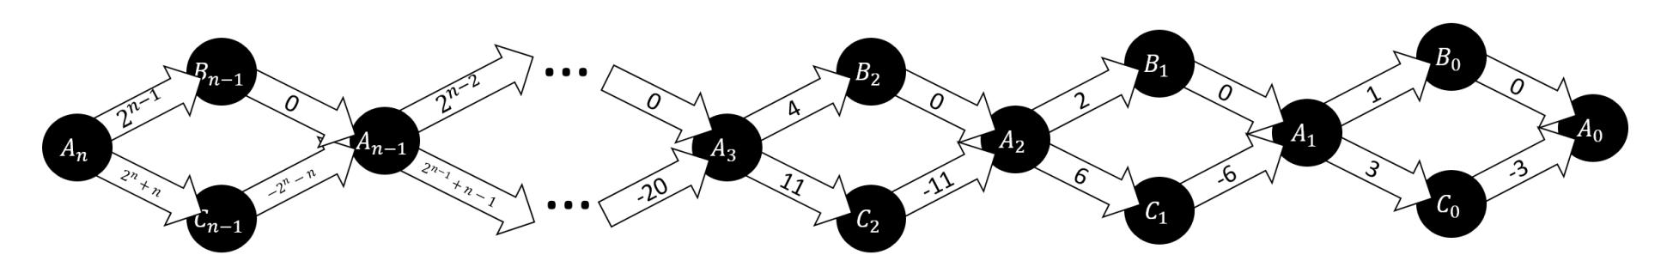
\includegraphics[scale=0.35]{Dijkstra_negative}
  \end{center}

  That is, $A_0$ has no outgoing neighbors and the adjacency list for each other vertex is:

  \begin{itemize}
  \item
  $A_k: (B_{k-1},2^{k-1}),(C_{k-1},2^k + k)$
  \item
  $B_k: (A_{k},0)$
  \item
  $C_k: (A_{k}, -2^k - k)$ 
  \end{itemize}

  \begin{enumerate}[(a)]
  \item
  Let $maxdist(v)$ be the maximum dist value that $dist(v)$ is set to (besides $\infty$) after
  running Dijkstra's on $H(n)$ starting at $A_n$.

  Prove by induction that $maxdist(v)\leq 2^n+n$ for all $v\in H(n)$.

  \begin{proof}
    We proceed by induction on $n$. Since $A_0$ has no out going edge, $maxdist(A_0) = 0 \leq 2^n +
    n$ and the base case is done. Suppose $n \geq 1$. Since there is only one path to either $B_{n -
    1}$ or $C_{n - 1}$ from $A_n$, $maxdist(B_{n - 1}) = 2^{k - 1}$ and $maxdist(C_{n - 1}) = 2^{k}
    + k$, both of which are at most $2^n + n$. There are two possible paths, $A_nB_{n - 1}A_{n - 1}$
    and $A_nC_{n - 1}A_{n - 1}$, from $A_n$ to $A_{n - 1}$, each having weights $2^{n - 1}$ and $0$,
    respectively. Since $2^{n - 1} < 2^k + k$, $maxdist(A_{n - 1})$ would be set to $2^{n - 1}$. But
    then $2^{n - 1} < 2^n + n$, so the algorithm would prioritize $A_{n - 1}$ over $C_{n - 1}$. By
    induction,
    \[
      maxdist(v) \leq maxdist(A_{n - 1}) + (2^{n - 1} + n - 1) \leq 2^{n - 1} + (2^{n - 1} + n - 1) = 2^n + n - 1 \leq 2^n + n,
    \]
    for all $v \in H(n - 1)$. Hence, the inequality holds true for all $v \in H(n)$.
  \end{proof}

  \item
  Prove by induction that after running Dijkstra's on $H(n)$, starting at $A_n$, the vertex $A_0$
  has been ejected from the priority queue $2^n$ times. (You can use the previous part.)

  \begin{proof}
    We proceed by induction on $n$. For $n = 0$, $H(0)$ consists of a single vertex $A_0$ and thus
    the algorithm would only eject it once. Suppose $n \geq 1$. Since $dist(A_{n - 1})$ would
    initially be assigned $2^{n - 1} < 2^n + n$, $A_{n - 1}$ would be prioritised over $C_{n - 1}$.
    By (a), $maxdist(v) \leq 2^{n - 1} + n - 1$ for all $v \in H(n - 1)$. But then $2^{n - 1} + 2^{n
    - 1} + n - 1 = 2^n + n - 1 < 2^n + n$, so all vertices of subscripts less than $n - 1$ would be
    prioritised over $C_{n - 1}$. Hence, the process of the algorithm before revisiting $C_{n - 1}$
    is equivalent to running Dijkstra's algorithm on $H(n - 1)$, which would ejected $A_0$ $2^{n -
    1}$ times, by induction. But then after revisiting $C_{n - 1}$, the algorithm push $A_{n - 1}$
    back to the priority queue, and the remaining process is also equivalent to running Dijkstra's
    algorithm on $H(n - 1)$, which would eject $A_0$ another $2^{n - 1}$ times. Hence, $A_0$ would
    be ejected $2^n$ times in total.
  \end{proof}

  \item
  Give a lower bound for the runtime of Dijkstra's on this graph in $\Omega$ notation in terms of
  the number of vertices $N$.

  \begin{proof}
    Given $N$ vertices in the graph, there would be $(N - 1)/3$ diamonds. Thus, by (b), the
    algorithm would at least process $A_0$ $2^{(N - 1)/3}$ times, which has a lower bound of $\Omega(2^{N/3})$.
  \end{proof}
\end{enumerate}
\end{homeworkProblem}

\newpage

\begin{homeworkProblem}
  Suppose Dijkstra's algorithm is run on the following graph, starting at node $A$.
  \begin{center}
    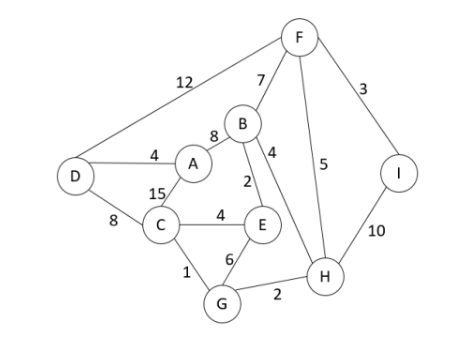
\includegraphics[scale=0.6]{Dijkstras}
  \end{center}
  \begin{enumerate}[(a)]
  \item
  Draw a table showing the intermediate distance values of all the nodes at each iteration of the
  algorithm.
  \begin{proof}
    Consider the following table:
    \begin{center}
      \begin{tabular}{|c|c|c|c|c|c|c|c|c|c|}
        \hline
        Iteration & $A$ & $B$ & $C$ & $D$ & $E$ & $F$ & $G$ & $H$ & $I$ \\
        \hline
        $0$ & $0$ & $\infty$ & $\infty$ & $\infty$ & $\infty$ & $\infty$ & $\infty$ & $\infty$ & $\infty$ \\
        \hline
        $1$ & $0$ & $8$ & $15$ & $4$ & $\infty$ & $\infty$ & $\infty$ & $\infty$ & $\infty$ \\
        \hline
        $2$ & $0$ & $8$ & $12$ & $4$ & $\infty$ & $16$ & $\infty$ & $\infty$ & $\infty$ \\
        \hline
        $3$ & $0$ & $8$ & $12$ & $4$ & $10$ & $15$ & $\infty$ & $12$ & $\infty$ \\
        \hline
        $4$ & $0$ & $8$ & $12$ & $4$ & $10$ & $15$ & $16$ & $12$ & $\infty$ \\
        \hline
        $5$ & $0$ & $8$ & $12$ & $4$ & $10$ & $15$ & $13$ & $12$ & $\infty$ \\
        \hline
        $6$ & $0$ & $8$ & $12$ & $4$ & $10$ & $15$ & $13$ & $12$ & $22$ \\
        \hline
        $7$ & $0$ & $8$ & $12$ & $4$ & $10$ & $15$ & $13$ & $12$ & $22$ \\
        \hline
        $8$ & $0$ & $8$ & $12$ & $4$ & $10$ & $15$ & $13$ & $12$ & $18$ \\
        \hline
        $9$ & $0$ & $8$ & $12$ & $4$ & $10$ & $15$ & $13$ & $12$ & $18$ \\
        \hline
      \end{tabular}
    \end{center}
  \end{proof}
  \item
  Draw the shortest path tree.
  \begin{center}
    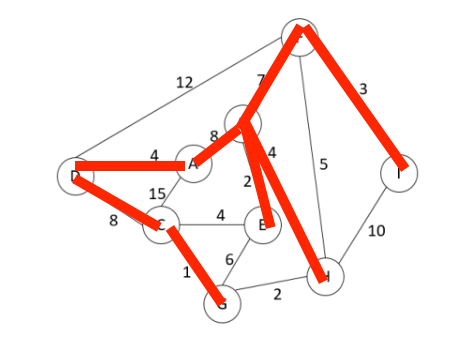
\includegraphics[scale=0.6]{Dijkstras_tree}
  \end{center}
  \end{enumerate}
\end{homeworkProblem}
\end{document}